% 西北农林科技大学科技类及IT类课程论文文档类(LaTeX模板)
\documentclass{nwafucoursepaper}

% 载入需要的宏包
% % =========浮动体增强宏包=========
% \usepackage{floatrow}
% \floatsetup[figure]{objectset=centering, margins=centering}

% % ========处理标题的宏包=========
% \usepackage[labelsep=quad]{caption}
% \usepackage{varioref}
% \usepackage{subfig}

% =========引号宏包=========
\usepackage{csquotes}

%%% Local Variables:
%%% mode: latex
%%% TeX-master:"../main.tex"
%%% End:

% 进行必要的设置
% ====================================================================================
% cquotes宏包的中文引号样式
% ====================================================================================
\DeclareQuoteStyle{zhquotestyle}% style name
    {\symbol{"201C}}% opening outer mark
    {\symbol{"201D}}% closing outer mark
    {\symbol{"2018}}% opening inner mark
    {\symbol{"2019}}% closing inner mark

\setquotestyle{zhquotestyle}

% ====================================================================================
% 改变表格字体
% ====================================================================================
\BeforeBeginEnvironment{tabular}{\small}%

%%% Local Variables:
%%% mode: latex
%%% TeX-master:"../main.tex"
%%% End:

% 专用术语宏命令进行必要的设置
% ====================================================================================
% 西北农林科技大学各单位名称
% ====================================================================================
\newcommand{\nwafu}{西北农林科技大学}
\newcommand{\cie}{信息工程学院}

% ============自定义专有名词命令============
\newcommand{\cl}{\texttt{C}语言}
\newcommand{\ccpp}{\texttt{C/C++}}
\newcommand{\win}{\texttt{Windows}}
\newcommand{\ide}{\texttt{IDE}}
\newcommand{\gcc}{\texttt{GCC}}
\newcommand{\gpp}{\texttt{G++}}
\newcommand{\gnu}{\texttt{GNU}}
\newcommand{\cb}{\texttt{Code::Blocks}}
\newcommand{\mgww}{\texttt{MinGW}}
\newcommand{\mgw}{\texttt{MinGW32}}
\newcommand{\mgwww}{\texttt{MinGW-w64}}
\newcommand{\lumos}{\texttt{Linux}、\texttt{Unix}、\texttt{Mac OS}}
\newcommand{\unix}{\texttt{UNIX}}
\newcommand{\lnx}{\texttt{Linux}}
\newcommand{\mk}{\texttt{make}}
\newcommand{\ph}{\texttt{Path}}
\newcommand{\cmdd}{\texttt{cmd}}
\newcommand{\gdb}{\texttt{gdb}调试器}
\newcommand{\vside}{\texttt{Visual Studio}}
\newcommand{\mfile}{\texttt{Makefile}}
\newcommand{\tgt}{\texttt{target}}
\newcommand{\prqt}{\texttt{prerequisites}}
\newcommand{\cbv}{\texttt{17.12}}
\newcommand{\db}{\texttt{DEBUG}}
\newcommand{\dbger}{\texttt{Debugger}}
\newcommand{\cdb}{\texttt{cdb}调试器}
\newcommand{\gdbcmd}{\texttt{(gdb)}}
\newcommand{\bug}{\texttt{BUG}}
\newcommand{\ieee}{\texttt{IEEE754}标准}
\newcommand{\ascii}{\texttt{ASCII}}
\newcommand\vararg{变长形参列表}
\newcommand\varargfun{\vararg{}函数}
\newcommand{\cg}{\texttt{CGraph2D} 图形库}
\newcommand{\git}{分布式版本控制系统\texttt{Git}}
\newcommand{\github}{\texttt{Github}平台}
% ====================================


%%% Local Variables:
%%% mode: latex
%%% TeX-master:"../main.tex"
%%% End:

% % % 用于排版LaTeX代码并同时输出结果的环境定义(若无此需要,可以不加载)
% % \usepackage{tcolorbox}
\usepackage{accsupp}  % PDF accessibility support

\tcbuselibrary{skins, minted, xparse}

% make line numbers unable to be selected
% ref: https://liam.page/2013/11/04/LaTeX-listings-copy/
\ExplSyntaxOn
\newcommand\emptyaccsupp[1]{
  \BeginAccSupp{ActualText={}} #1 \EndAccSupp{}
}

\renewcommand\theFancyVerbLine{
  \emptyaccsupp{
    \textcolor[rgb]{0.5, 0.5, 1.0}{
      \scriptsize\arabic{FancyVerbLine}
    }
  }
}
\ExplSyntaxOff

\makeatletter
\tcbset{
  % see tcbminted.code.tex, def of "minted options"
  % minted options/.store in=\kvtcb@minted@options,
  minted options app/.code=\appto\kvtcb@minted@options{,#1}
}
\makeatother

% define new option
\tcbset{
  example options/.style={
    skin=bicolor,
    colbacklower=white,
    fonttitle=\sffamily,
    minted options app={
      % line numbers
      linenos,
      numberfirstline=true,
      stepnumber=2,
      numbersep=5pt,
      % break point
      breakbefore=\\,
    }
  },
  example title/.style 2 args={
    title=Example\ifblank{#1}{}{ #1}\ifblank{#2}{}{: #2}
  }
}


% new env: example
% #1 - <kv list>, tcb-listing options
% #2 - <token list>, title
\makeatletter
\NewTCBListing[auto counter]{example}{ O{} m }{
  example options,
  example title={\thetcbcounter}{#2},
  #1
}
\makeatother

% new env: example*
% like example, except that it is un-numbered
\NewTCBListing{example*}{ O{} m }{
  example options,
  example title={}{#2},
  #1
}

% % % 用于排版LaTeX命令代码的环境定义(若无此需要,可以不加载)
% % \RequirePackage{tcolorbox}
\tcbuselibrary{documentation}

\ExplSyntaxOn
\makeatletter

% #1 = tcb options
% #2 = clist of 3-tuple, "{name}{arg}{desc}, {}{}{}, ..."
\NewDocumentEnvironment{docCommands}{ O{} m }
  {
    \tcbset{#1}
    \begin{tcb@manual@entry}
    \tcb_doc_heads:n {#2}
    \nobreak\tcbset{before~ upper=}
    \kvtcb@doc@body@command@before
    \ignorespaces
  }
  {
    \ifvmode\else\unskip\fi
    \kvtcb@doc@body@command@after
    \end{tcb@manual@entry}
  }

% to use \seq_pop_right:NN
\seq_new:N \l_tcb_heads_seq

% #1 = clist of 3-tuple, "{csname}{arg}{desc}, {}{}{}, ..."
\cs_new:Nn \tcb_doc_heads:n
  {
    \seq_set_from_clist:Nn \l_tcb_heads_seq {#1}
    \seq_pop_left:NN \l_tcb_heads_seq \l_tmpa_tl
    \exp_after:wN \tcb_doc_head:nnnn \l_tmpa_tl 
      {after~ skip=0pt, enlarge~ bottom~ by=0pt}
    \seq_pop_right:NN \l_tcb_heads_seq \l_tmpa_tl
    \seq_map_inline:Nn \l_tcb_heads_seq
      {
        \tcb_doc_head:nnnn ##1 
          {before~ skip=0pt, after~ skip=0pt, enlarge~ bottom~ by=0pt}
      }
    \exp_after:wN \tcb_doc_head:nnnn \l_tmpa_tl 
      {before~ skip=0pt, enlarge~ bottom~ by=-0.2\baselineskip}
  }

% #1 = command csname
% #2 = arg spec
% #3 = command description
% #4 = tcb options
\cs_new:Nn \tcb_doc_head:nnnn
  {
    \begin{tcb@doc@head}{doc@head@command, #4}
    \strut
    \tcb@Print@Com{#1}\tcb@index@Com{#1}
    \protected@edef\@currentlabel{\noexpand\tcb@cs{#1}}\label{com:#1}
    {\ttfamily #2}
    \gdef\kvtcb@doc@description{#3}%  result of \tcbset{doc description=#3}
    \tcb@doc@do@description
    \end{tcb@doc@head}
  }

\makeatother
\ExplSyntaxOff

\endinput

% usage
\begin{docCommands}
{
  {menu}
    {\oarg{input sep}\marg{menu sequence}}
    {\oarg{input sep} defaults to |>|},
  {directory}
    {\oarg{input sep}\marg{menu sequence}}
    {\oarg{input sep} defaults to |/|},
  {keys}
    {\oarg{input sep}\marg{menu sequence}}
    {\oarg{input sep} defaults to |+|}
}
  content
\end{docCommands}

%% ----------------------------
%% begin: original definitions
%%   from tcbdocumentation.code.tex
%%   link https://github.com/T-F-S/tcolorbox/blob/master/tex/latex/tcolorbox/tcbdocumentation.code.tex
%% ----------------------------

%\newenvironment{docCommand}[3][]{\tcbset{#1}%
%  \begin{tcb@manual@entry}%
%  \begin{tcb@doc@head}{doc@head@command}%
%  \tcb@Print@Com{#2}\tcb@index@Com{#2}\protected@edef\@currentlabel{\noexpand\tcb@cs{#2}}\label{com:#2}{\ttfamily #3}%
%  \tcb@doc@do@description%
%  \end{tcb@doc@head}\nobreak\tcbset{before upper=}\kvtcb@doc@body@command@before\ignorespaces}%
%  {\ifvmode\else\unskip\fi\kvtcb@doc@body@command@after\end{tcb@manual@entry}}
%
%\newenvironment{tcb@manual@entry}{\begin{list}{}{%
%  \setlength{\leftmargin}{\kvtcb@doc@left}%
%  \setlength{\itemindent}{0pt}%
%  \setlength{\itemsep}{0pt}%
%  \setlength{\parsep}{0pt}%
%  \setlength{\rightmargin}{\kvtcb@doc@right}%
%  }\item}{\end{list}}
%
%\newtcolorbox{tcb@doc@head}[1]{blank,colback=white,colframe=white,
%  code={\tcbdimto\tcb@temp@grow@left{-\kvtcb@doc@indentleft}%
%        \tcbdimto\tcb@temp@grow@right{-\kvtcb@doc@indentright}},
%  grow to left by=\tcb@temp@grow@left,%
%  grow to right by=\tcb@temp@grow@right,
%  sidebyside,sidebyside align=top,
%  sidebyside gap=-\tcb@w@upper@real,
%  phantom=\phantomsection,%
%  enlarge bottom by=-0.2\baselineskip,#1}

%% ----------------------------
%% end: original definitions
%% ----------------------------

% 乱数假文宏包
\usepackage{zhlipsum}
\usepackage{hyperref}
\usepackage{listings}
\lstset{
  numbers=left,
  stepnumber=1,
  showspaces=false,
  showtabs=false,
  breaklines=true,
  showstringspaces=false,
  breakatwhitespace=true,
  commentstyle=\color{green},
  keywordstyle=\color{blue},
  stringstyle=\color{red},
  basicstyle=\ttfamily,
  moredelim=[il][\textcolor{pgrey}]{$$},
  moredelim=[is][\textcolor{pgrey}]{\%\%}{\%\%}
}

\title{\bfseries\sffamily E-Exercise学习答题网站项目报告}
\author{\zihao{4} \fangsong 封钰震(1951362)\\\fangsong 信息管理与信息系统 \\\small \songti 管理科学与工程系}
\date{\small \today}

% 摘要内容
\begin{abstract}
\end{abstract}
% 关键词内容(用英文","分割)
\keywords{}

%biblatex宏包的参考文献数据源加载方式
\addbibresource[location=local]{bib/example.bib}
\begin{document} %在document环境中撰写文档
% 排版标题
\maketitle
\thispagestyle{empty}
% 排版摘要
% \makeabstract

\section{前言}

本网站可以通过IP地址进行访问,登录界面的URL为\url{http://47.103.73.100:8081/ExerciseOnline/user/toLogin}。在答辩完成后本网站所有源代码将在GitHub上进行开源,遵循MIT License开源协议,网址为\url{https://github.com/Feng-Yz/Java-Homework/tree/main/FinalProject/Exercise-Web-Online}。

\section{工作描述}

本人通过十个左右日夜的努力,使用Spring Boot+Thymeleaf+MyBatis框架实现了一个名为“E-Exercise”的学习答题网站,主要包括用户模块、知识模块和习题模块,并将其部署在云服务器上。在知识模块,实现了知识间依赖关系的构建,以Markdown标记语言作为知识模板;在习题模块,实现了习题作答、习题批改、习题推荐等功能,同时在原始Markdown语法的基础上,面向选择题拓展了该标记语言,使得用户能够较方便地添加习题。本网站没有采用XML标记语言作为知识和内容的模板,考虑到的是用户需求,因为不熟悉XML的用户较难使用,因此采用广受大众喜爱的简单易学的Markdown标记语言。

\section{需求分析}

项目需要完成一个基于知识和习题数据的课程学习、检验、测试的平台,具备的学习评价、学习过程记录、学习路径推荐等功能,同时建立知识模板和习题模板。因此,本人根据这些需求,结合实际情况,设计了如下功能:

\subsection{基本功能}

网站的基本功能包括\textbf{用户注册}与\textbf{用户登录},另也需要有验证码防止恶意行为,注册时系统也需要会查看邮箱是否已经被注册(若已经被注册,需要进行报警)。

\subsection{知识功能}

对于学生用户来说,需要\textbf{查看课程列表},进入课程页面后需要\textbf{查看知识清单}和\textbf{查看知识内容},知识内容需要适应不同的格式(例如代码、公式、图片等),也需要\textbf{显示学习进度}反映自己学习情况。

对于管理员与教师来说,需要\textbf{添加课程}、\textbf{添加知识}、\textbf{修改课程}、\textbf{修改知识}等功能。添加和修改知识时,也需要为知识\textbf{设置前置依赖知识}。同时,为了服务管理员和教师添加知识,网站也需要\textbf{上传图片},图片上传后,可以在知识中使用图片。

\subsection{习题功能}

对于学生用户来说,进入知识清单后需要对应知识\textbf{查看习题},也可以查看系统的\textbf{推荐习题}。学生需要在习题页面\textbf{回答习题}。对于选择题和判断题等客观题,系统需要\textbf{自动批改};其他情况需要交由教师批改。学生可在\textbf{作答记录}中查看自己的\textbf{作答情况}。

对于管理员与教师来说,可以\textbf{添加习题}、\textbf{修改习题}、\textbf{批改习题}。习题内容也需要适应不同的格式。

\subsection{功能总览}

根据以上的需求分析,本网站的所有主体功能如图\ref{功能总览图}所示。

\begin{figure}[htp]
  \centering
  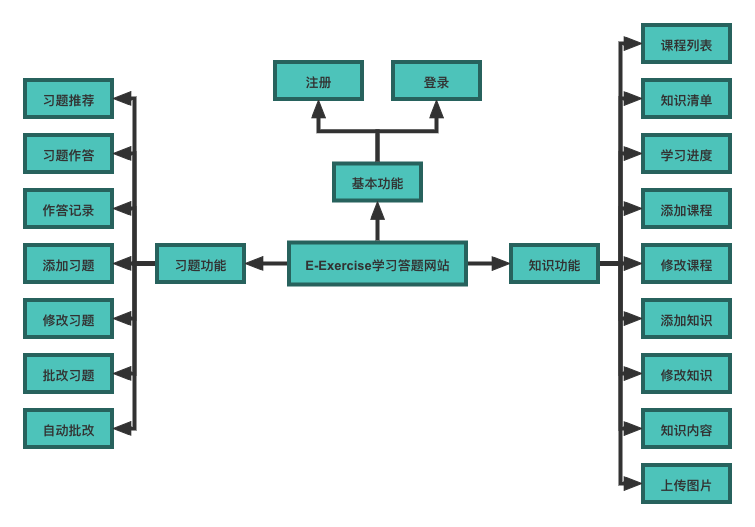
\includegraphics[width=0.8\textwidth]{功能总览图.png}
  \caption{功能总览}
  \label{功能总览图}
\end{figure}

\section{实现解析}

\subsection{整体框架}

本系统使用Spring Boot+Thymeleaf+MyBatis实现各个模块,数据库管理系统采用的是远程MySQL,Web服务器使用Tomcat,使用Git作为版本控制器,集成开发环境为IDEA教育版(其中集成了Maven作为项目管理工具)。如表\ref{environment}所示。

\begin{table}[htp]
  \centering
  \begin{tabular}{|c|c|}
  \hline
  内容        & 工具          \\ \hline
  Web框架     & Spring Boot \\ \hline
  Java模板引擎  & Thymeleaf   \\ \hline
  Java持久化框架 & MyBatis     \\ \hline
  数据库管理系统   & 远程MySQL     \\ \hline
  Web服务器     & Tomcat     \\ \hline
  版本控制      & Git         \\ \hline
  项目管理      & Maven       \\ \hline
  集成开发环境    & IDEA Edu    \\ \hline
  \end{tabular}
  \caption{开发环境}
  \label{environment}
\end{table}

\subsection{项目结构}

在Spring Boot项目的文件夹中,主要包括:
\begin{enumerate}
  \item \verb|src/main/java|文件夹,其中为本项目的Java源代码;
  \item \verb|src/main/resources|文件夹,其中为本项目的静态资源与配置文件;
  \item \verb|src/test|文件夹,其中为测试代码。
\end{enumerate}

\verb|src/main/java/com/Yuzhen/ExerciseOnline/|的内容具体如下:
\begin{itemize}
    \item \verb|auxiliary/|:辅助类,主要包括一些辅助函数,例如:对知识和习题模板的处理、对上传文件重命名等;
    \item \verb|entity/|:数据库实体类;
    \item \verb|controller/|:控制器类,用于处理Http请求、配置URL映射等;
    \item \verb|service/|:用于处理业务逻辑;
    \item \verb|repository/|:用于数据访问的接口;
    \item \verb|NoLoginException.java|:用于处理未登录异常;
    \item \verb|GlobalExceptionHandleController.java|:用于处理其他异常;
    \item \verb|ExerciseOnlineApplication.java|:主类。
\end{itemize}

\verb|src/main/resources/|的内容具体如下:
\begin{itemize}
    \item \verb|application.properties|:应用程序的配置文件;
    \item \verb|mappers/|:Mybatis的XML映射文件;
    \item \verb|static/|:网页静态资源;
    \item \verb|templates/|:网页模板。
\end{itemize}

Spring Boot项目中处理用户访问请求的流程如图\ref{Spring Boot流程图}所示,其中用户通过页面进行访问或请求,交由Controller处理,Controller调用Service层的业务逻辑,Service层再通过Repository(也称Mapper层或DAO层)的接口与数据库进行交互,传入传出数据。

\begin{figure}[htp]
  \centering
  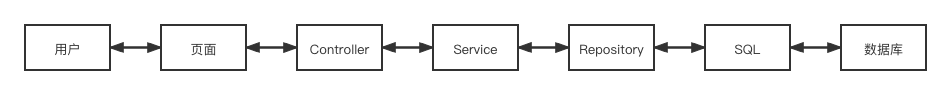
\includegraphics[width=\textwidth]{springboot.png}
  \caption{Spring Boot流程图}
  \label{Spring Boot流程图}
\end{figure}

\subsection{数据库设计}

根据需求分析,设计出符合一定范式的数据库结构,分为7张表,每张表的内容如表\ref{tables}所示。表之间的关系如图\ref{ERD}所示。

\begin{table}[htp]
  \centering
  \begin{tabular}{|c|c|}
  \hline
  表名                    & 介绍          \\ \hline
  user                  & 储存用户信息      \\ \hline
  subject               & 储存课程信息      \\ \hline
  knowledge             & 储存知识信息      \\ \hline
  exercise              & 储存习题信息      \\ \hline
  answer                & 储存用户的答题信息   \\ \hline
  knowledge\_dependency & 储存知识间的依赖关系  \\ \hline
  image                 & 储存用户上传的图片信息 \\ \hline
  \end{tabular}
  \caption{数据库表结构}
  \label{tables}
  \end{table}

\begin{figure}[htp]
  \centering
  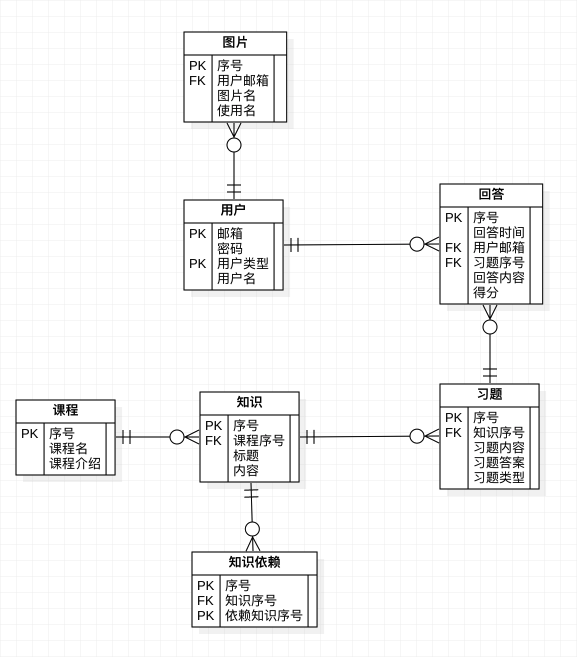
\includegraphics[width=0.6\textwidth]{ERD.png}
  \caption{ER图}
  \label{ERD}
\end{figure}

\subsection{功能解析}

对于网站的登录、注册、课程列表、知识清单等大多数功能,只涉及对数据库的增删改查,故不进行具体介绍,本小节只介绍部分重要功能。

\subsubsection{习题推荐}

学生可以通过“小试牛刀”界面查看系统推荐的习题,系统推荐习题的规则如下:
\begin{enumerate}
  \item 推荐过去完成的习题中最高分不超过85分的习题;
  \item 对于未产生进度的知识点,查看其前置依赖知识是否进度不低于75\%,若其中存在进度低于75\%的知识,则不推荐;反之,则推荐;
  \item 对于产生进度的知识点,推荐用户未做过的习题。
\end{enumerate}
从所有的可推荐习题中,随机选择15题进行推荐。

\subsubsection{知识模板}

知识模板主要使用的是Markdown标记语言,例如,
\begin{lstlisting}
  # 这是一级标题

  ## 这是二级标题

  ### 这是三级标题

  > 这是引用块

  - 这是无序列表
  - 这是无序列表

  1. 这是有序列表
  2. 这是有序列表
  3. 这是有序列表

  ```
  这是代码块
  ```

  $ $
  这是公式块
  $ $

  也可以使用`行内代码`与$行内公式$。
\end{lstlisting}

前端可以使用Marked插件渲染Markdown标记的内容,也可以使用MathJax插件渲染数学公式,但MathJax渲染得到的界面有些丑陋,因此网站使用Zhihu提供的接口,将Tex公式转化为图片。要实现这样的目标,需要对知识内容进行词法分析,寻找到其中由\verb|$$|包围的数学公式,并将其转化为向Zhihu提供的接口发送的请求内容。辅助类\verb|Auxiliary|的\verb|modifyContent|函数实现了这样的修改。最终网页的呈现结果如图\ref{knowledge_math}所示。

\begin{figure}[htp]
  \centering
  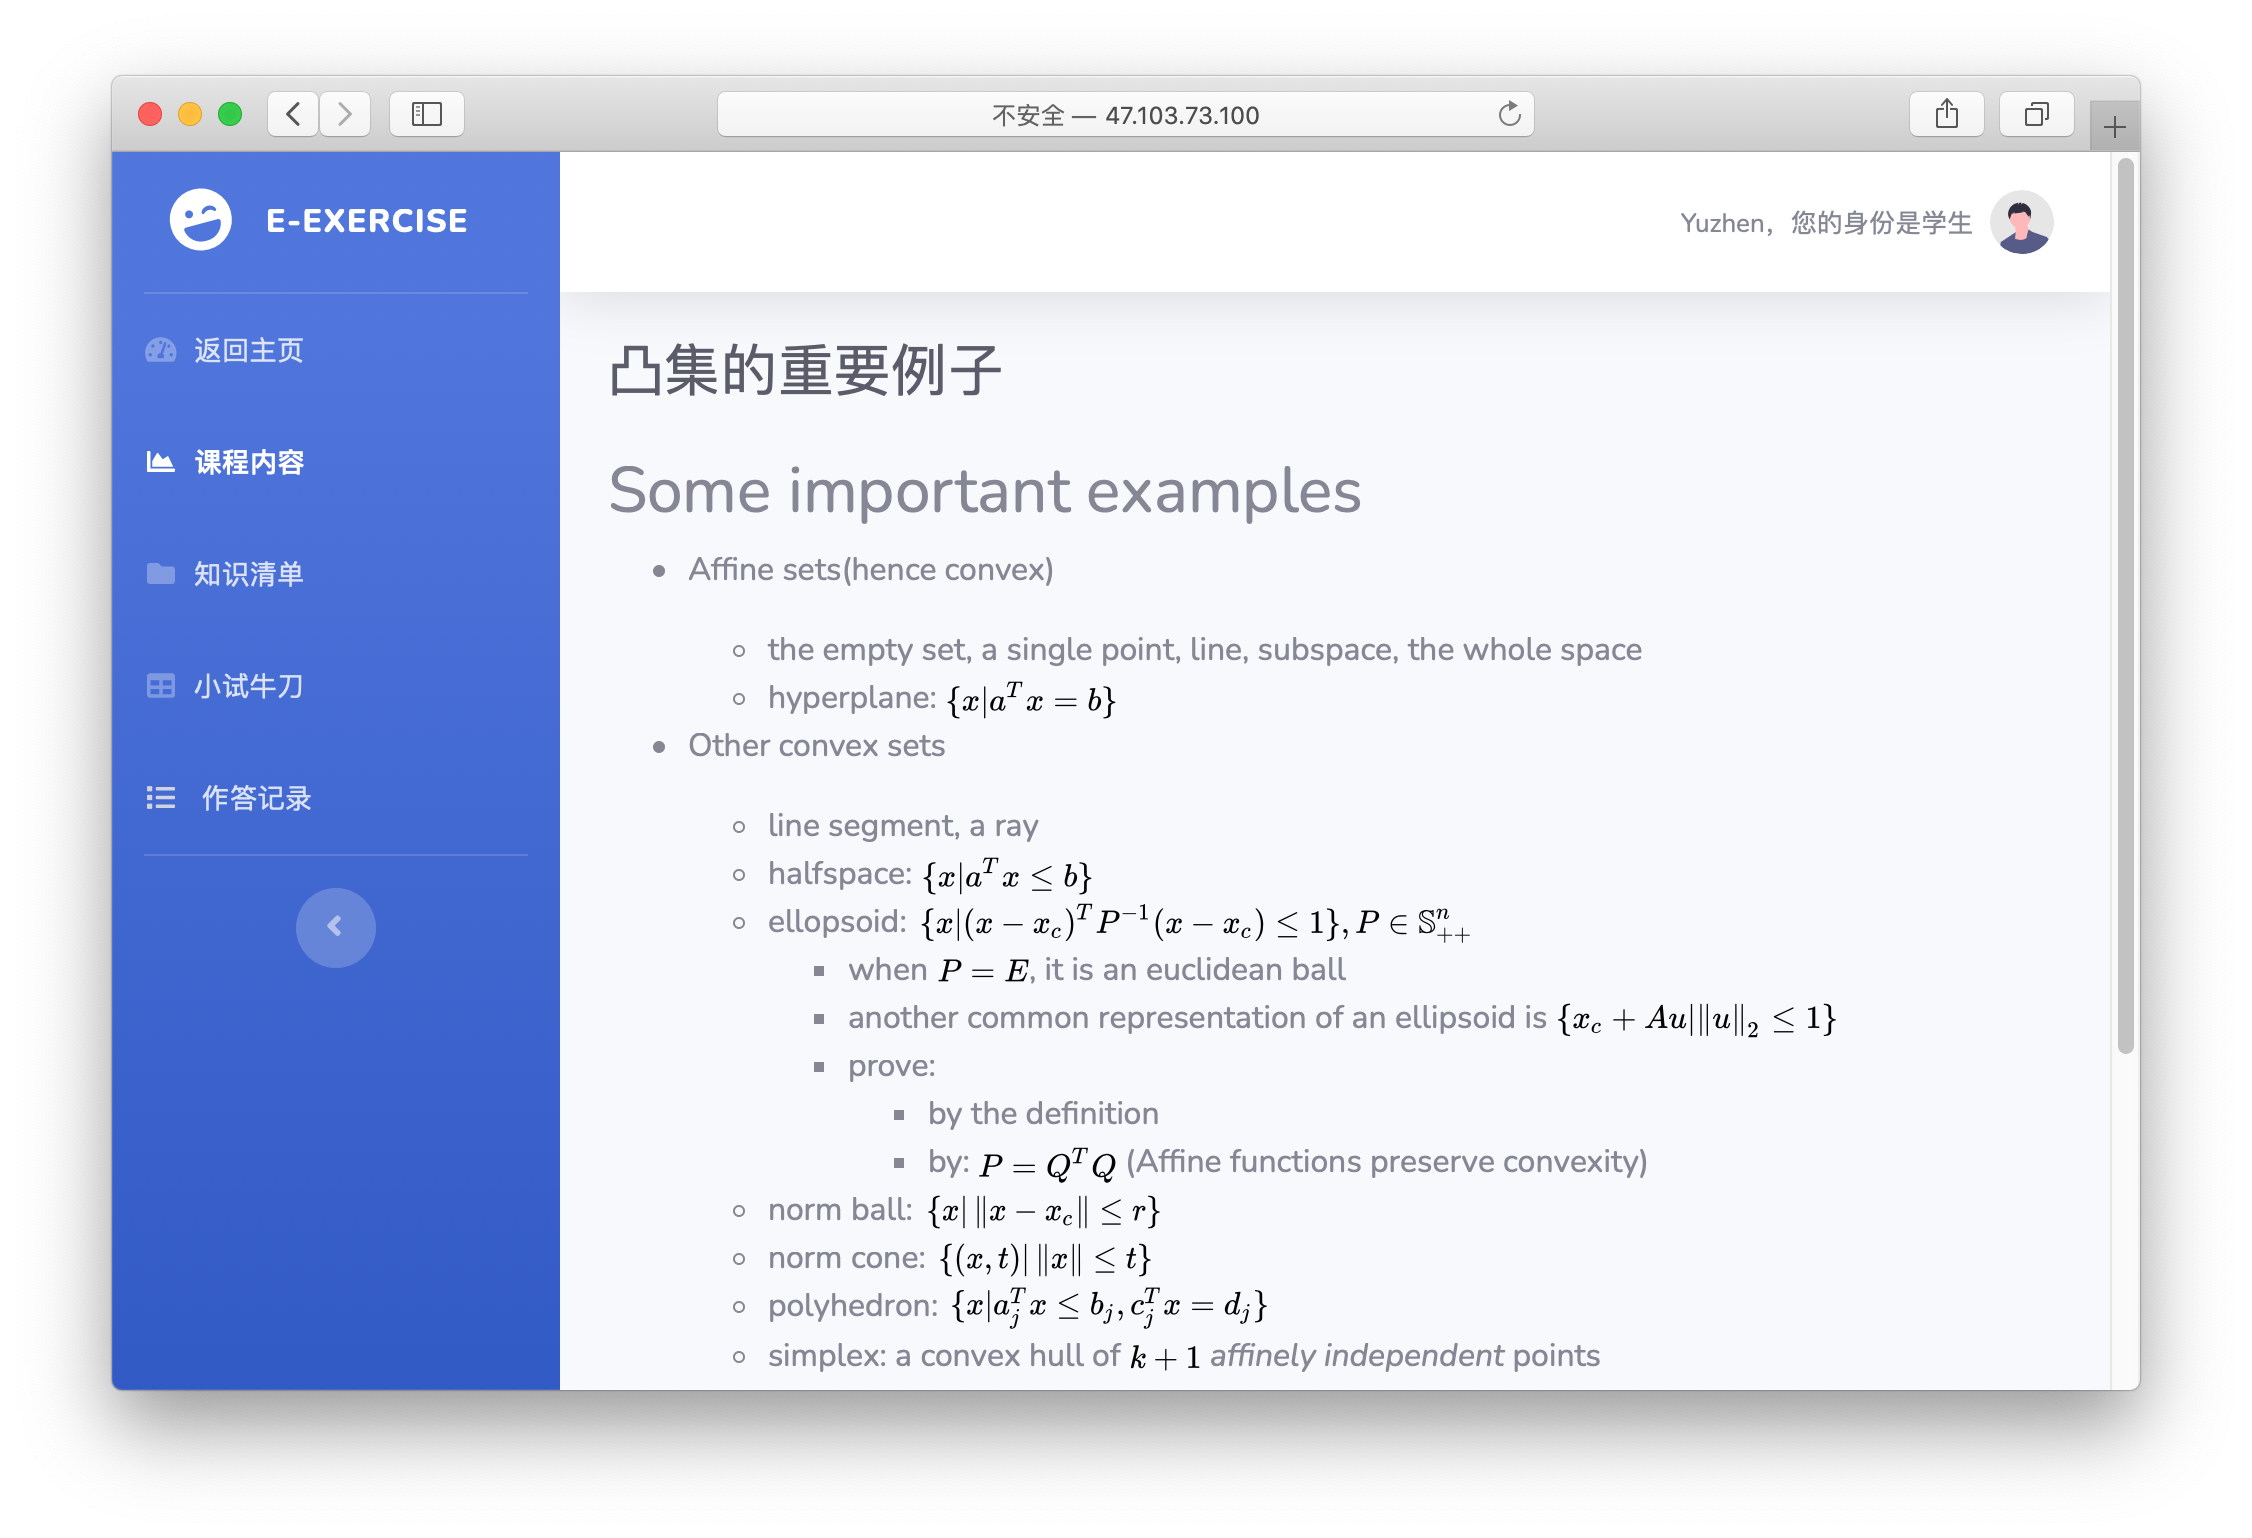
\includegraphics[width=0.8\textwidth]{knowledge_math.png}
  \caption{知识页面}
  \label{knowledge_math}
\end{figure}

\subsubsection{习题模板}

\begin{figure}[htp]
  \centering
  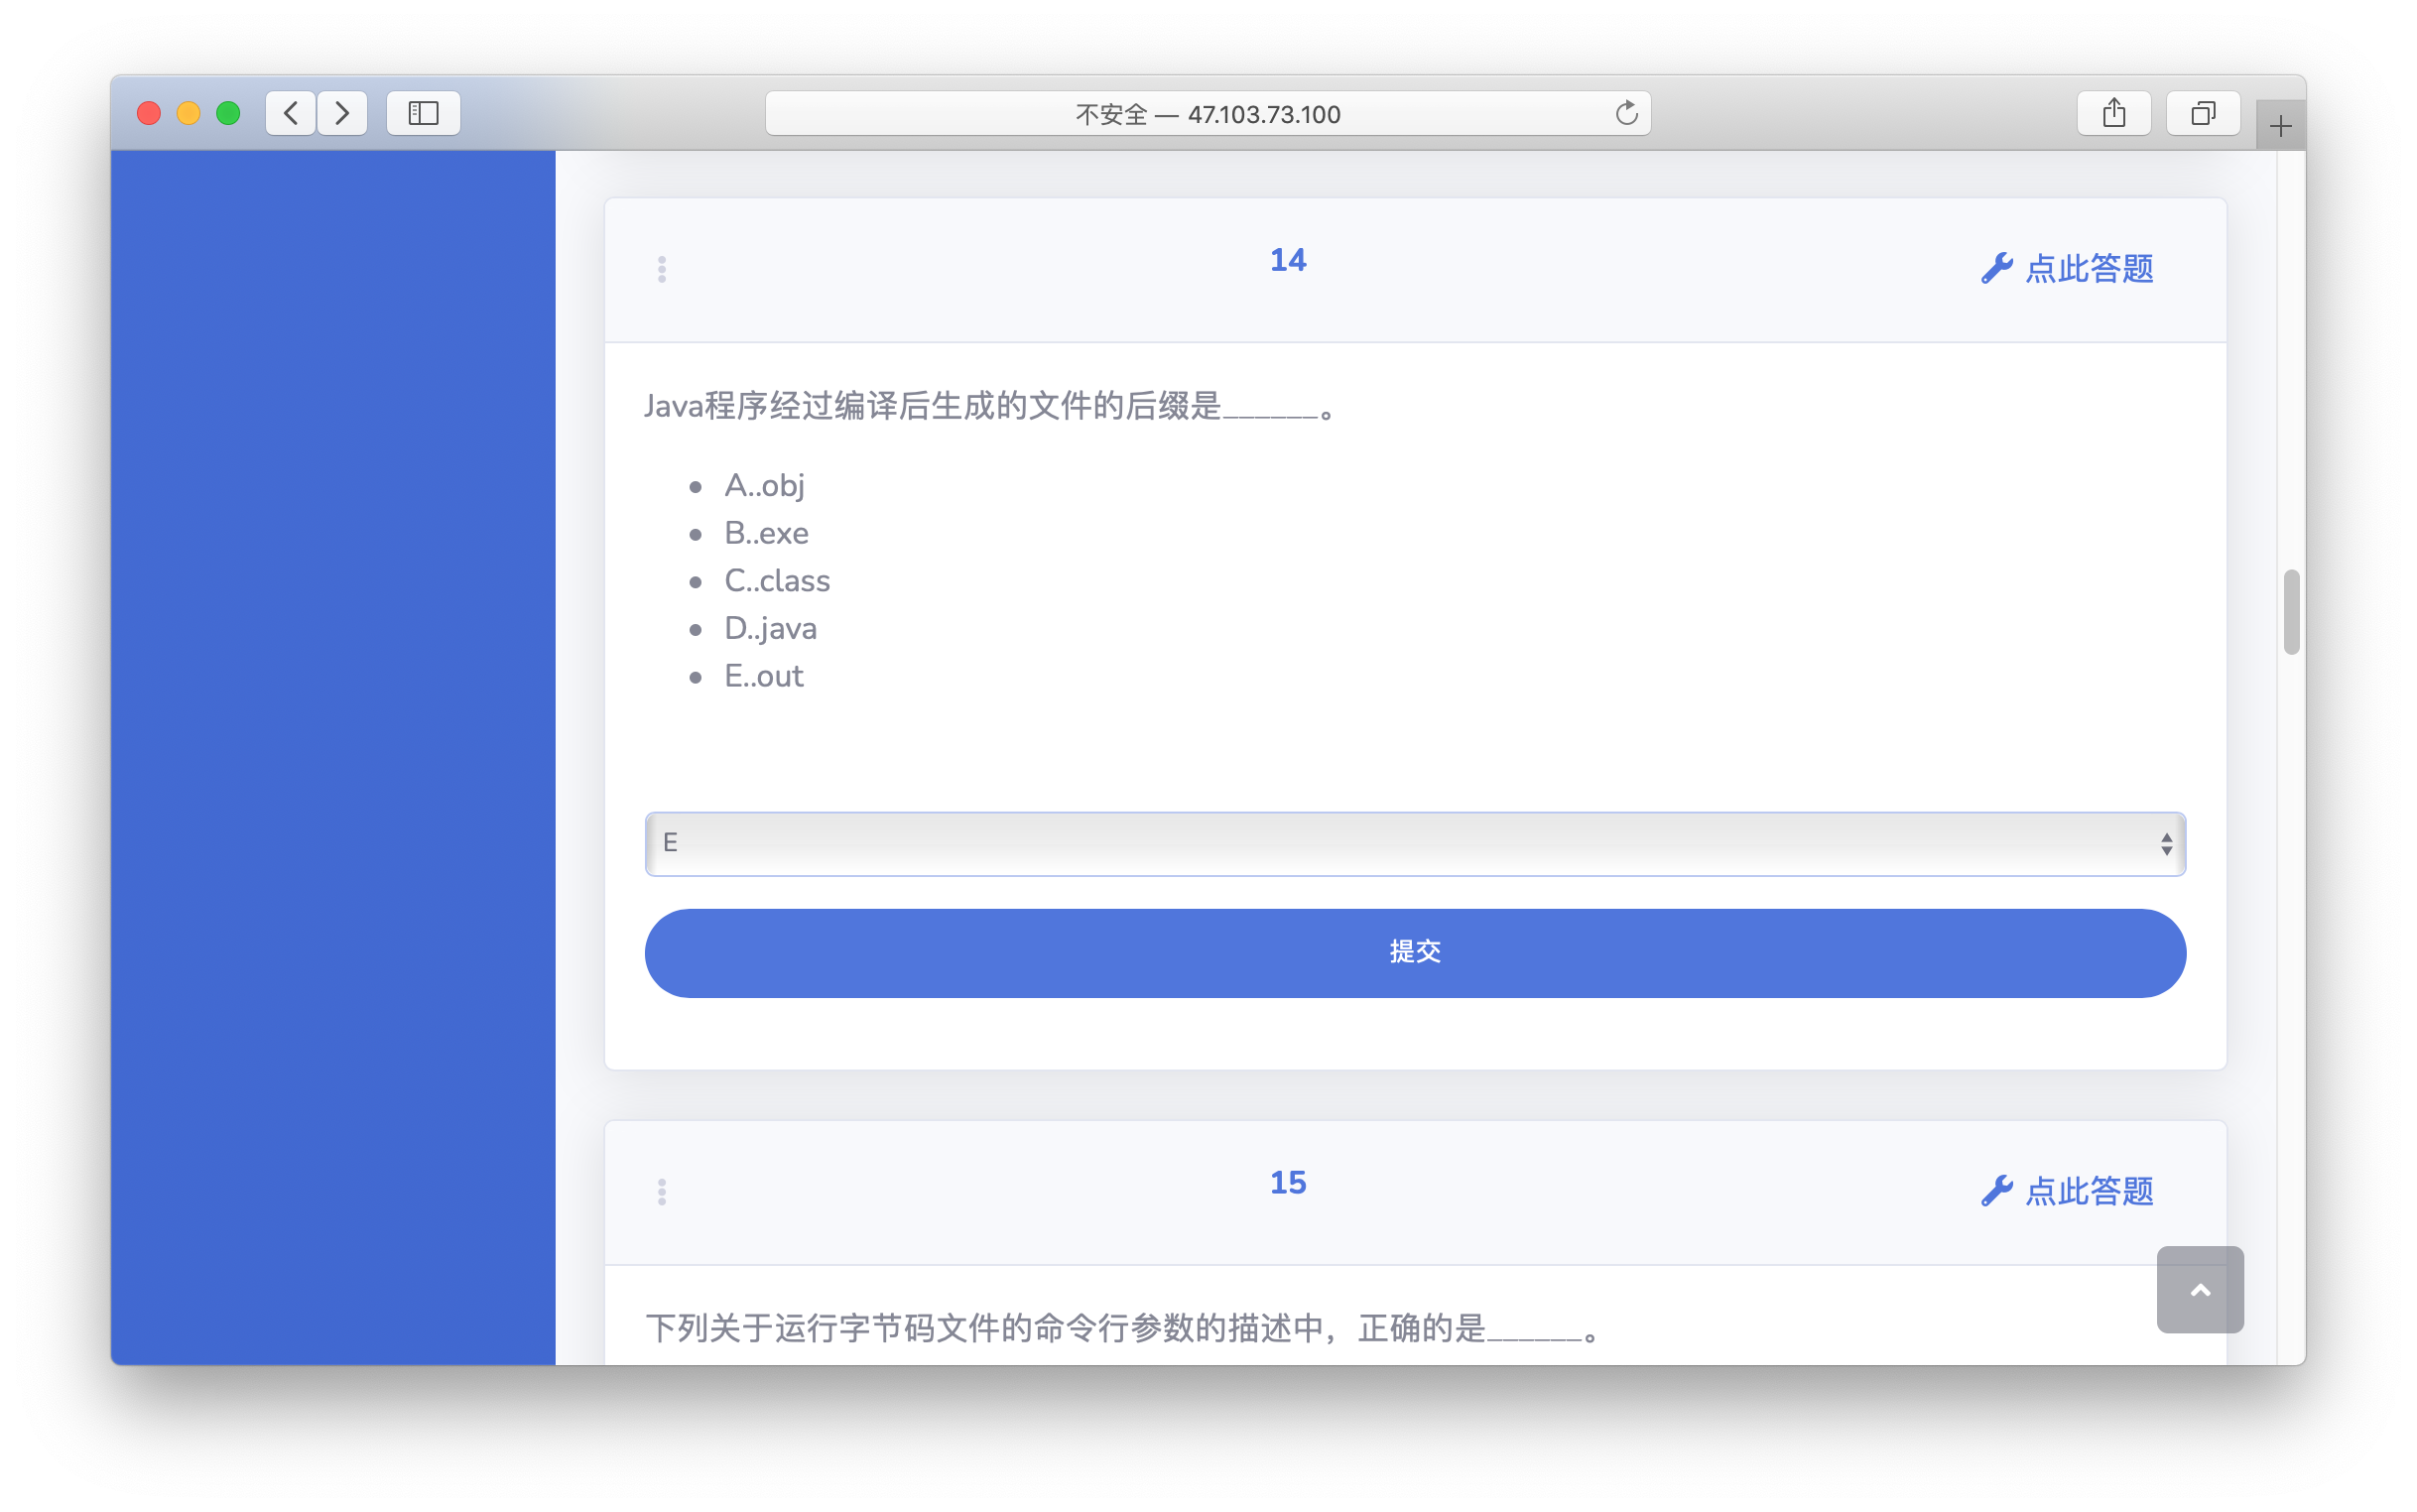
\includegraphics[width=0.8\textwidth]{answer_exercise.png}
  \caption{回答习题}
  \label{answer_exercise}
\end{figure}

习题模板也采用Markdown标记语言作为模板,在此基础上,为选择题增添了标签。模板中用\verb|<opt>|标记选择题的选项,例如,图\ref{answer_exercise}中的选择题内容如下:
\begin{lstlisting}
  Java程序经过编译后生成的文件的后缀是______。
  <opt>A..obj
  <opt>B..exe
  <opt>C..class
  <opt>D..java
  <opt>E..out
\end{lstlisting}
此时,若有超过4个选项的习题,系统也能自动识别,并在用户答题时提供对应数量的选项,如图\ref{answer_exercise}所示便自动提供了\verb|E|选项。

\subsubsection{自动批改}

该功能是由数据库的触发器实现的,插入数据到\verb|answer|表时,触发器被触发。若该回答对应的题目为客观题且事先输入了标准答案,则新插入的记录中的分数会根据是否与答案相同而给分。触发器的代码如下:
\lstset{language=sql}
\begin{lstlisting}
  DELIMITER $$
  CREATE Trigger judge BEFORE INSERT ON answer FOR EACH ROW
  BEGIN
      DECLARE right_answer TEXT;
      DECLARE exercise_type INT;
      SELECT answer, type INTO right_answer, exercise_type FROM exercise WHERE exercise.id=NEW.exercise_id;
      IF ISNULL(right_answer) != 1 AND LENGTH(TRIM(right_answer)) != 0 THEN
          IF exercise_type = 1 OR exercise_type = 2 THEN
              IF right_answer = NEW.answer THEN
                  SET NEW.is_right = 100;
              ELSE
                  SET NEW.is_right = 0;
              END IF;
          END IF;
      END IF;
  END
  DELIMITER ;
\end{lstlisting}

\section{小结与回顾}

本项目通过Spring Boot+Thymeleaf+MyBatis框架,基本实现了要求的所有功能,并保证了一定的美观与用户友好性。

通过这次开发,我学习了Spring Boot这样一个主流框架,也进一步了解了Java项目管理与依赖建立、Web项目部署、XML文件语法及相关操作、HTML+CSS+JS等前端工具、MyBatis、Thymeleaf等,受益匪浅。当然,也有一些不足之处,例如在某些功能上用户体验可能不足。

\section{致谢}

最后,要感谢缪洲同学在我学习Spring Boot的初期提供了一些指导,感谢JetBrains提供便利的IDE工具、感谢GitHub提供有效的代码托管服务和开源平台、感谢Stack Overflow等论坛的网友提供十分有用的交流、感谢Alibaba提供廉价的学生服务器、也特别要感谢赵思璇同学提供Java习题数据。

% 打印参考文献表
% \printbibliography[heading=bibliography,title=参考资料]
\end{document}
